\centering\singlespacing
\tikzset{every picture/.style={line width=0.75pt}} %set default line width to 0.75pt        
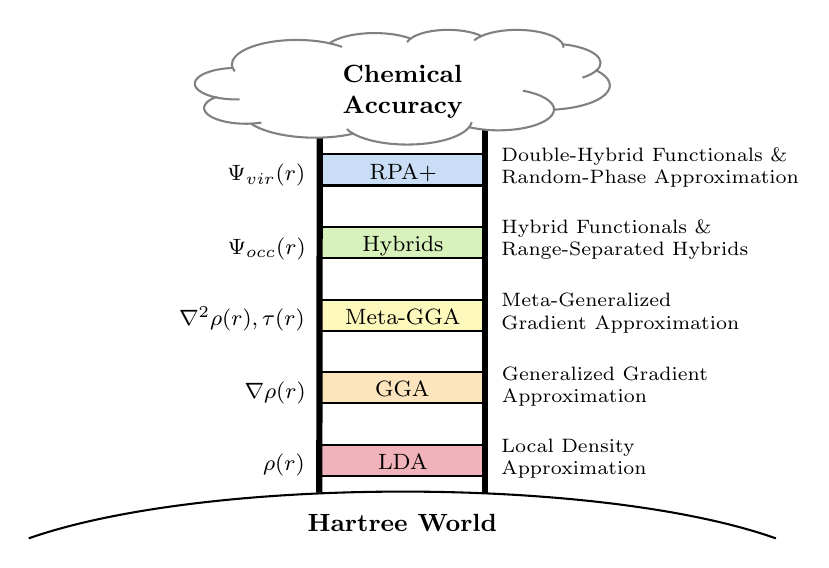
\begin{tikzpicture}[x=0.75pt,y=0.75pt,yscale=-1,xscale=1]
%Curve Lines [id:da86891233878799] 
\draw    (29,246) .. controls (114.03,216.08) and (303.78,215.83) .. (389,246) ;
%Shape: Rectangle [id:dp6440602598272736] 
\draw  [fill={rgb, 255:red, 241; green, 179; blue, 187 }  ,fill opacity=1.0 ] (169,201) -- (249,201) -- (249,216) -- (169,216) -- cycle ;
%Shape: Rectangle [id:dp16390793343447418] 
\draw  [fill={rgb, 255:red, 252; green, 228; blue, 189 }  ,fill opacity=1.0 ] (169,166) -- (249,166) -- (249,181) -- (169,181) -- cycle ;
%Shape: Rectangle [id:dp44785830951060834] 
\draw  [fill={rgb, 255:red, 253; green, 248; blue, 187 }  ,fill opacity=1.0 ] (169,131) -- (249,131) -- (249,146) -- (169,146) -- cycle ;
%Shape: Rectangle [id:dp38853804770808686] 
\draw  [fill={rgb, 255:red, 216; green, 242; blue, 188 }  ,fill opacity=1.0 ] (169,96) -- (249,96) -- (249,111) -- (169,111) -- cycle ;
%Shape: Rectangle [id:dp45002736761667594] 
\draw  [fill={rgb, 255:red, 201; green, 222; blue, 246 }  ,fill opacity=1.0 ] (169,61) -- (249,61) -- (249,76) -- (169,76) -- cycle ;
%Straight Lines [id:da9515996496239052] 
\draw [line width=2.25]    (169.26,32.59) -- (169,224) ;
%Straight Lines [id:da24533370255825981] 
\draw [line width=2.25]    (249,36) -- (249,224) ;
%Shape: Cloud [id:dp33766008859162566] 
\draw  [color={rgb, 255:red, 128; green, 128; blue, 128 }  ,draw opacity=1 ][fill={rgb, 255:red, 255; green, 255; blue, 255 }  ,fill opacity=1 ] (127.2,19.2) .. controls (125.59,14.74) and (130.88,10.33) .. (140.82,7.83) .. controls (150.76,5.34) and (163.61,5.2) .. (173.92,7.47) .. controls (177.57,4.88) and (184.26,3.09) .. (191.95,2.65) .. controls (199.65,2.2) and (207.45,3.15) .. (213,5.21) .. controls (216.1,2.86) and (222.21,1.28) .. (229.15,1.03) .. controls (236.09,0.79) and (242.88,1.91) .. (247.1,3.99) .. controls (252.72,1.5) and (261.66,0.45) .. (270.06,1.3) .. controls (278.45,2.15) and (284.79,4.74) .. (286.33,7.95) .. controls (293.22,8.66) and (298.96,10.46) .. (302.06,12.88) .. controls (305.16,15.3) and (305.33,18.12) .. (302.52,20.59) .. controls (309.3,23.91) and (310.88,28.34) .. (306.68,32.22) .. controls (302.48,36.1) and (293.13,38.85) .. (282.11,39.44) .. controls (282.03,43.08) and (276.73,46.43) .. (268.24,48.18) .. controls (259.75,49.93) and (249.41,49.82) .. (241.2,47.89) .. controls (237.7,52.26) and (227.85,55.47) .. (215.91,56.14) .. controls (203.97,56.81) and (192.08,54.82) .. (185.36,51.03) .. controls (177.14,52.9) and (167.27,53.43) .. (157.99,52.52) .. controls (148.7,51.61) and (140.78,49.32) .. (136.01,46.18) .. controls (127.6,46.55) and (119.48,44.91) .. (115.66,42.07) .. controls (111.85,39.24) and (113.16,35.81) .. (118.94,33.49) .. controls (111.44,31.83) and (107.62,28.53) .. (109.46,25.32) .. controls (111.3,22.11) and (118.39,19.71) .. (127.03,19.37) ; \draw  [color={rgb, 255:red, 128; green, 128; blue, 128 }  ,draw opacity=1 ] (118.94,33.49) .. controls (122.48,34.27) and (126.57,34.63) .. (130.65,34.51)(136.01,46.18) .. controls (137.76,46.1) and (139.49,45.94) .. (141.13,45.69)(185.36,51.03) .. controls (184.13,50.33) and (183.09,49.58) .. (182.28,48.8)(241.2,47.89) .. controls (241.84,47.1) and (242.25,46.28) .. (242.43,45.45)(282.11,39.44) .. controls (282.19,35.57) and (276.34,32.02) .. (267.07,30.32)(302.52,20.59) .. controls (301.01,21.91) and (298.72,23.08) .. (295.82,24.01)(286.33,7.95) .. controls (286.59,8.48) and (286.71,9.02) .. (286.69,9.57)(247.1,3.99) .. controls (245.7,4.61) and (244.55,5.31) .. (243.67,6.05)(213,5.21) .. controls (212.25,5.77) and (211.69,6.37) .. (211.33,6.99)(173.92,7.47) .. controls (176.1,7.95) and (178.12,8.53) .. (179.93,9.2)(127.2,19.2) .. controls (127.42,19.81) and (127.77,20.42) .. (128.25,21.01) ;
% Text Node
\draw (209.25,30.75) node  [font=\small] [align=left] {\textbf{Chemical}\\\textbf{Accuracy}};
% Text Node
\draw (255.25,196.75) node [anchor=north west][inner sep=0.75pt]  [font=\scriptsize] [align=left] {Local Density \\Approximation};
% Text Node
\draw (255.5,162) node [anchor=north west][inner sep=0.75pt]  [font=\scriptsize] [align=left] {Generalized Gradient \\Approximation};
% Text Node
\draw (255.25,126.5) node [anchor=north west][inner sep=0.75pt]  [font=\scriptsize] [align=left] {Meta-Generalized \\Gradient Approximation};
% Text Node
\draw (255.25,91) node [anchor=north west][inner sep=0.75pt]  [font=\scriptsize] [align=left] {Hybrid Functionals \&\\ Range-Separated Hybrids};
% Text Node
\draw (209.5,75.5) node [anchor=south] [inner sep=0.75pt]  [font=\footnotesize] [align=left] {RPA+};
% Text Node
\draw (209.25,214.5) node [anchor=south] [inner sep=0.75pt]  [font=\footnotesize] [align=left] {LDA};
% Text Node
\draw (209,179.25) node [anchor=south] [inner sep=0.75pt]  [font=\footnotesize] [align=left] {GGA};
% Text Node
\draw (209.25,144.55) node [anchor=south] [inner sep=0.75pt]  [font=\footnotesize] [align=left] {Meta-GGA};
% Text Node
\draw (209.25,111.4) node [anchor=south] [inner sep=0.75pt]  [font=\footnotesize] [align=left] {Hybrids};
% Text Node
\draw (255.25,56.5) node [anchor=north west][inner sep=0.75pt]  [font=\scriptsize] [align=left] {Double-Hybrid Functionals \&\\ Random-Phase Approximation};
% Text Node
\draw (163.5,217.6) node [anchor=south east] [inner sep=0.75pt]  [font=\footnotesize]  {$\rho (\bm{r})$};
% Text Node
\draw (164,182.6) node [anchor=south east] [inner sep=0.75pt]  [font=\footnotesize]  {$\nabla \rho (\bm{r})$};
% Text Node
\draw (163.5,147.6) node [anchor=south east] [inner sep=0.75pt]  [font=\footnotesize]  {$\nabla ^{2} \rho (\bm{r}) ,\tau (\bm{r})$};
% Text Node
\draw (164,113.6) node [anchor=south east] [inner sep=0.75pt]  [font=\footnotesize]  {$\Psi _{\text{occ}}(\bm{r})$};
% Text Node
\draw (163.75,77.85) node [anchor=south east] [inner sep=0.75pt]  [font=\footnotesize]  {$\Psi _{\text{vir}}(\bm{r})$};
% Text Node
\draw (209,244.15) node [anchor=south] [inner sep=0.75pt]  [font=\small] [align=left] {\textbf{Hartree World}};
\end{tikzpicture}
\onehalfspacing